\documentclass[]{report}
\usepackage{graphicx}
\usepackage{hyperref}
\graphicspath{{images/}}

% Title Page
\title{Applications of Hill Climbing To Find A Minimum Within Complex Functions}
\author{Jesse Roland}


\begin{document}
\maketitle

\begin{abstract}
	\fontsize{14}{16}\selectfont
	Hill climbing is a greedy algorithm used to find minimum's and maximum's within a function. For three dimensional planes, this is accomplished by incrementing and decrementing \textbf{X} and \textbf{Y} by a defined step size. Depending on whether the goal is searching for a minimum or maximum, the hill climbing algorithm will advance if the resulting \textbf{Z} value is either less than or greater than the former value, respectively.
	
	For functions such as \begin{math}
	Z = X^2 + Y^2
	\end{math} a simple hill climbing algorithm can easily find the minimum, no matter where it starts. This is because that there is a clear constant path towards the minimum. However, if there is a ridge, attaining the solution can become more complicated. A ridge is defined as a position where the plane increases and decreases, forming an independent hill inside of the function. For complex functions, this is a common occurrence, and by the nature of the hill climbing algorithm, it will get stuck, and no longer be able to explore further for a better minimum/maximum.
	
	In this paper variations of the hill climbing algorithm will be tested on a complex function with such ridges. These variations are \textbf{hill climbing with random restarts} and \textbf{simulated annealing}. Each will be tested against the following function:\\
	\begin{math}
	Z=\frac{\sin{(x^2+3y^2)}}{0.1+r^2}+(x^2+5y^2)*\frac{\exp{(1-r^2)}}{2},r=\sqrt{x^2+y^2}
	\end{math}\\The goal is to find the minimum.
	
\end{abstract}

\chapter{Understanding The Problem}
	
	The problem assigned has designated the domain and range of the function beforehand. The search space is \begin{math}
		{\{-2.5 <= \textbf{X} <= 2.5\}} 
	\end{math} and \begin{math}
		{\{-2.5 <= \textbf{Y} <= 2.5\}} 
	\end{math} 
	
	Due to the constraints, the search space is discrete. This means that within the space a global minimum can be found, where \textbf{global} is defined as the entire space specified by the domain and range. Here is a graphical representation of the function in three dimensional space.\\
	\fontsize{6}{8}\selectfont
	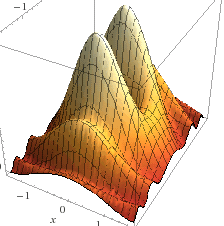
\includegraphics{hill}\\Wolfram Alpha LLC. 2009. Wolfram Alpha. \url{http://goo.gl/ZCcd83} (access March 15, 2016).\\
	\fontsize{12}{14}\selectfont
	Within this space, there exists some global minimum.

\chapter{Application: Standard Hill Climbing}
	\section{Implementation}
	The first function to test will be the standard hill climbing algorithm. The implementation of the algorithm used can be described by the following steps:
	\begin{description}
		\item[1.] Assign the starting \textbf{X} and \textbf{Y} coordinates, and calculate the \textbf{Z} value.
		\item[2.] Increase \textbf{X} by the step size.
		\item[3.] If the new \textbf{Z} value is less than the former, set \textbf{X} as the new coordinate.
		\item[4.] Decrease \textbf{X} by the step size.
		\item[5.] If the new \textbf{Z} value is less than the former, set \textbf{X} as the new coordinate.
		\item[6.] Increase \textbf{Y} by the step size.
		\item[7.] If the new \textbf{Z} value is less than the former, set \textbf{Y} as the new coordinate.
		\item[8.] Decrease \textbf{Y} by the step size.
		\item[9.] If the new \textbf{Z} value is less than the former, set \textbf{Y} as the new coordinate.
		\item[10.] If any of steps \textbf{3},\textbf{5},\textbf{7},\textbf{9} are true, return to step \textbf{2}.
		\item[11.] Return the current \textbf{Z} value.	
	\end{description}
	The idea behind this is that the function will attempt all possible directions, and by it's greedy nature, will take all routes as soon as it finds a valid path. At a glance, the algorithm appears flawed. By increasing then immediately decreasing, an instinct reaction to this is that the algorithm will go back and forth between two points infinitely. However, it must be noted that the new value needs to be less than it's former; therefore, the algorithm will be unable to back track and will not get stuck between two points. It should also be noted that the algorithm will not take a step beyond it's bounds, meaning that \textbf{X} and \textbf{Y} will not exceed -2.5 and 2.5
	\section{Testing}
	The problem does not specify a starting point to solve the problem. As a result, the \textbf{X minimum} and the \textbf{Y minimum} are used as starting coordinates for exploration.\\\\
	\textbf{Step size = 1}\\
	Under this condition, the algorithm explored nothing. All negative steps were beyond the minimum range, and were not explored. The two positive steps had a larger \textbf{Z} value than the former established by the original coordinates.
	Minimum value calculated: \textbf{-0.010314167895642582}\newpage
	\textbf{Step size = 0.1}\\
	This test was able to take three steps, where it increased \textbf{X}, increased \textbf{Y}, and then decreased \textbf{X}. The following is a graphic of the test:\\
	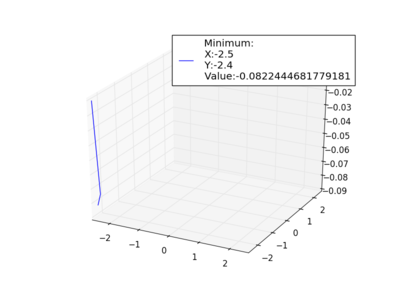
\includegraphics{hc01}\\Fortunately, the algorithm was able to actually progress, unfortunately, it did not progress very far.\newpage
	\textbf{Step size = 0.01}\\
	This condition enabled the algorithm to take twelve steps, however the result was still not impressive.\\
	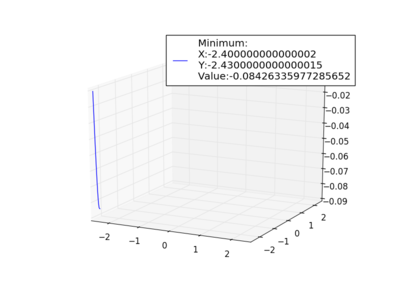
\includegraphics{hc001}\\
	\textbf{Notice:} The decimal numbers are slightly different than what they should be, and will continue to be so for certain test cases. This is attributed to the floating point arithmetic used in python, the language the algorithm's were written in. More details on this phenomena can be found in the \textbf{Analysis and Conclusion} chapter.\newpage
	\textbf{Step Size = 0.001}\\
	This case took a significantly larger number of steps, reaching 326, however it's simplicity and greedy nature led it to a similar conclusion as the other test cases.\\
	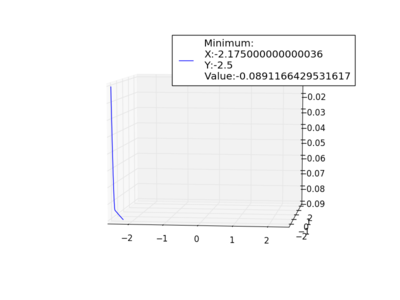
\includegraphics{hc0001}
	
	\chapter{Application: Hill Climbing Random Restart}
	\section{Implementation}
	The premise of hill climbing with random restarts is to follow the standard procedure of climbing, but to conduct it such that random \textbf{X} and \textbf{Y} coordinates are chosen, and explored. The smallest minimum is then taken from all the searches, and then returned. Procedurally, the following steps are to be taken:
	\begin{description}
		\item[1.] For the number of random restarts, randomly generate an arbitrary set of \textbf{X} and \textbf{Y} coordinates.
		\item[2.] For each coordinate, apply the hill climbing algorithm.
		\item[3.] Find the path with the smallest minimum
		\item[4.] Return that value as the minimum.
	\end{description}
	From the \textbf{standard hill climbing} tests, a step size of \textbf{0.001} proved to be the most successful at navigating the search space, therefore, that will be the step size used.\\
	\newpage
	\section{Testing}
	\textbf{Restarts = 1}\\
	This test was similar to a standard hill climb, with the exception that rather than beginning at the lowest possible range and domain values, it chose a random location in the space. As a result, the algorithm already appears to have improved more so than \textbf{standard hill climbing}.\\
	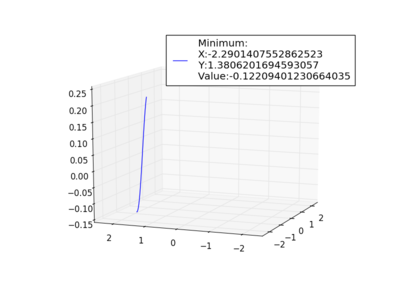
\includegraphics{hcr1}\newpage
	\textbf{Restarts = 10}\\
	This test case demonstrated greater promise to find the minimum, where it was able to explore many points in the search space.\\
	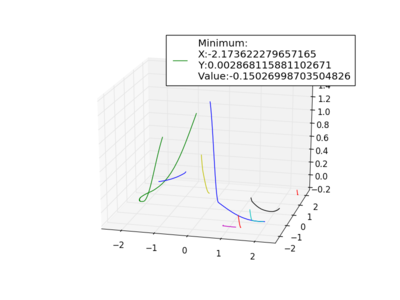
\includegraphics{hcr10}\\
	\textbf{Restarts = 100}\\
	An interesting qualitative trait of this approach is that it's data is beginning to resemble the original search space in shape.\\
	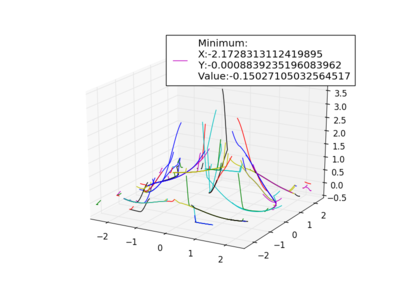
\includegraphics{hcr100}\newpage
	\textbf{Restarts = 1000}\\
	Another qualitative note is that the number of \textbf{restarts} can be set to rather large numbers and be processed in a reasonable amount of time.\\
	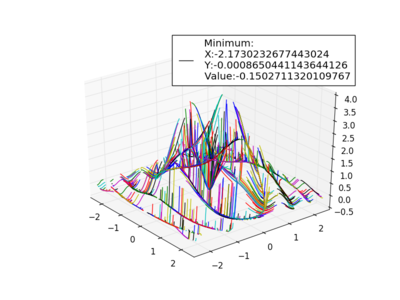
\includegraphics{hcr1000}\\
	\textbf{Restarts = 10000}\\
	This test looks promising in adequately searching the entirety of the function.\\
	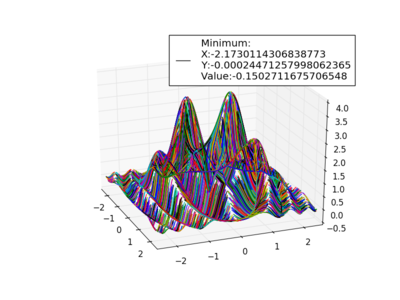
\includegraphics{hcr10000}
	\chapter{Application: Simulated Annealing}
	\section{Prerequisite}
	Simulated annealing is derived from the practice of metallurgy. When working with metals, the process of annealing requires heating a metal to a high temperature. The metal is then gradually cooled on a schedule. Once the metal is at room temperature again, it's molecular structure is better optimized to handle high heat.
	\section{Implementation}
	Simulated annealing uses this technique to find a minimum within a space. It starts at a high "temperature" and begins hill climbing. A higher temperature has a probability of the algorithm randomly taking an incorrect path. This notion can prevent the algorithm from getting stuck on a small ridge. However, larger ridges are more difficult for the algorithm to bypass. As the temperature is lowered, it also becomes less likely the algorithm will stray; this results in the algorithm reaching larger ridges, staying within them, and thus finding the global minimum of the function. An interesting behavior of this algorithm is that, similar to metal annealing, lowering the temperature more slowly can produce better results. The function for calculating the probability based on the temperature is the following:
	\begin{math}
	e^{\frac{F(new) - F(old)}{Temperature}}
	\end{math}\newpage
	The steps taken for accomplishing simulated annealing are the following:
	\begin{description}
		\item[1.] Begin \textbf{Standard Hill Climbing}\\
		\item[] While climbing:
		\item[2.] Apply the temperature function using the former and new \textbf{Z} value
		\item[3.] If the climb is valid, climb regardless of the temperature function.
		\item[4.] If the climb is invalid, but the temperature function allows it, climb anyways.
	\end{description}
	\textbf{Notice:} The project assigned for this research did not specify a parameter in the code to set the decrease in temperature, but rather how high the temperature is to be set. As a result, rather than modifying the rate of temperature change, the temperature itself will be changed, and decrease at a constant rate of \textbf{0.001} per iteration of \textbf{standard hill climbing}.\newpage
	\section{Testing}
	\textbf{Temperature = 1}\\
	An improvement on \textbf{standard hill climbing}, the algorithm appears to prevent itself from getting stuck on the first ridge.\\
	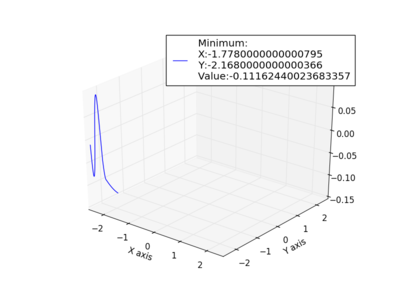
\includegraphics{sa1}\\
	\textbf{Temperature = 2}\\
	As expected, the algorithm was able to explore further.\\
	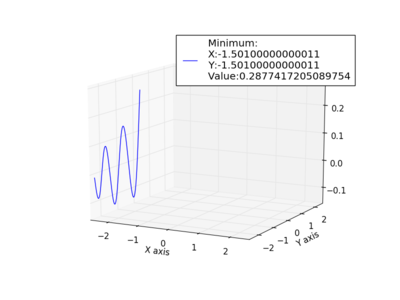
\includegraphics{sa2}\newpage
	\textbf{Temperature = 3}\\
	Here, the algorithm was able to find a strong path by being able to climb incorrectly.\\
	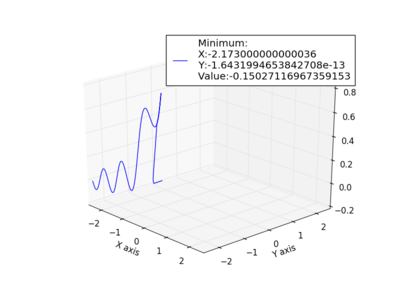
\includegraphics{sa3}\\
	\textbf{Temperature = 4}\\
	This test led to the same solution as the previous, but with a slightly varied path to get there.\\
	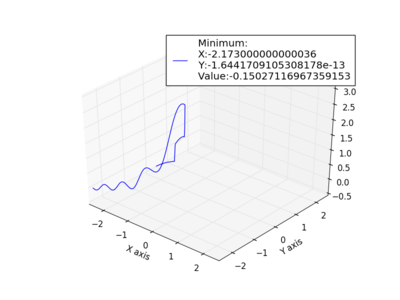
\includegraphics{sa4}
	
	\chapter{Analysis and Conclusion}
	\section{Analysis}
	The results produced by the three algorithms had similarities and differences; most had advantages and drawbacks as well.
	\subsection{Standard Hill Climbing}
	\textbf{Standard Hill Climbing} performed the worst out of all the algorithm's. It was unable to progress very far into the search space. This was expected, as the function had multiple ridges. The algorithm's best minimum was also the worst compared to the other two techniques used.
	\subsection{Hill Climbing With Random Restarts}
	This technique proved to be powerful for solving this particular problem. When the number of restarts was set high enough, it was able to cover so much area that it nearly represented the graphical representation of the function. 
	
	As stated during the tests, the algorithm was surprisingly fast. For the test case of \textbf{10000} random restarts, it was able to calculate the minimum in \textbf{19.635 seconds}. This figure was gained using the GNU/Linux \textbf{time} command when running the python script. This statistic was given from a computer with a \textbf{Intel Core i5-2520M}, no graphics card, and \textbf{7871 MB of RAM}. To ensure that the algorithm was the only variable in the test, no print functions were called.
	
	A reason this search was so successful can be attributed to the fact that the search space was small and finite. For this reason, the starting points were clustered, and able to cover a significant amount of the function. A second reason the algorithm performed so well is the actual geometry of the function. By observing the graphical representation, it can be seen that there are few small ridges, and a few comparably large ones. This meant that the algorithm did not get stuck as often, and was able to cover a large distance with each search. 
	
	One small disadvantage to note was that due to the pseudo-random nature of the algorithm, it would sometimes find a minimum that was smaller than the last test, when no parameters were changed.
	
	In it's best test, \textbf{Hill climbing with random restarts} calculated a minimum of \textbf{-0.1502711675706548}.
	
	\subsection{Simulated Annealing}
	This approach also proved to be able to search the space effectively, and was able to do so in significantly less time than \textbf{hill climbing with random restarts}.
	
	\textbf{simulated annealing} in it's best test case calculated a minimum value of \textbf{-0.15027116967359153}. Technically, this value was smaller than that given from \textbf{hill climbing with random restarts}, but it should be noted that floating point arithmetic in python can contain small rounding errors. This will be explained in the next subsection.
	
	An advantage that \textbf{simulated annealing} had over \textbf{hill climbing with random restarts} was certainty. Although \textbf{hill climbing with random restarts} was able to find an similar minimum in the test involving \textbf{10} restarts, when run multiples times it had cases where it failed to find a similar minimum. The same occurred when restarts were set to \textbf{100}. Although rare, out of \textbf{100000} runs of both test cases, simulated annealing never failed to find the minimum, and \textbf{hill climbing with random restarts} failed at least once when using \textbf{100} restarts.
	
	A disadvantage however, was coverage. \textbf{Simulated annealing} was able to find a similar minimum, but at the same time it did not explore as much as \textbf{hill climbing with random restarts}, the hill climb was able to cover the majority of the search space, while \textbf{simulated annealing} covered very little in comparison.
	
	\subsection{Possible Error To Consider}
	Looking back to the test cases, the resulting values were not always calculated entirely accurately. For example, in the third test of the \textbf{standard hill climbing} algorithm, the step size was set to \textbf{0.01}. The starting coordinates were the \textbf{X} and \textbf{Y} minimum, \textbf{-2.5}. Mathematically speaking, when exploring the search space the algorithm could not have been a value such as the ones produced, where \textbf{X = -2.40000000000000002}. If the step size was only \textbf{0.01}, then it is impossible to add or subtract the step size from \textbf{-2.5} and reach the produced result. This was a result of floating point arithmetic. The language used, \textbf{Python}, had small rounding errors, this is a commonly known occurrence in computer science, and for this reason the best outputs between \textbf{simulated annealing} and \textbf{hill climbing with random restarts} are considered equivalent in this paper.\newpage
	
	\section{Conclusion}
	Due to the outstandingly poor performance of \textbf{standard hill climbing}, \textbf{simulated annealing} and \textbf{hill climbing with random restarts} are the only two to even be considered efficient solutions for finding the minimum of the function. Therefore, they will be the only two discussed.
	
	In terms of coverage, \textbf{hill climbing with random restarts} was far superior to \textbf{simulated annealing}. As previously stated, the algorithm was able to cover the majority of the search space.
	
	However in terms of reliability, \textbf{simulated annealing} showed to be much more consistent at solving the problem.  \textbf{hill climbing with random restarts} was able to find the minimum, but on rare occasions failed. \textbf{Simulated annealing} never failed no matter how many times it was run.
	
	Although sometimes failing, \textbf{hill climbing with random restarts} could be corrected, if given enough restarts. When given \textbf{10000} restarts, it never failed a test either. Also, as explained in section \textbf{5.1.2}, it did not take a particularly unreasonable amount of time for the algorithm to explore at \textbf{10000} restarts.
	
	For this reason, and because it can cover so much more space and have a better certainty, \textbf{hill climbing with random restarts} is the superior algorithm for finding the minimum of the function given.
	
\end{document}          
